\chapter{Testing}
\chapterlabel{tests}

Testing is indispensible during language development to validate that your
language definition corresponds to your mental design of the language. Automatic
testing is also indispensible for maintenance of your language; does your
language extension still support all the original use cases?

In this chapter we discuss how to test a Spoofax language definition using the
SPT testing language \cite{KatsVV11,KatsVV11a} and using plain example files.
You can find the code for this chapter in example project \LanguageRepoRef{LanguageA}.
The project defines a language with the name \texttt{LangA}.

\section{Testing with SPT}

We start by adding a \texttt{test/} directory to our project and in that
directory we create \texttt{test/expr-syntax.spt} to contain tests for the
expressions in our language.

An SPT test module first declares its name and the language that its tests are
about:

\begin{verbatim}
  module expr-syntax
  language LangA
\end{verbatim}

Next it declares the start symbol with respect to which the tests will be
parsed:

\begin{verbatim}
  start symbol Expr
\end{verbatim}

For each kind of program fragment that should be tested separately, such as
expressions here, the corresponding non-terminal symbol should be declared as
start symbol in the SPT file \emph{and} in the syntax definition, as we will see
in the next chapter.

After these initial declarations follows a series of tests of the form

\begin{verbatim}
  test <name> [[ <fragment> ]] <property>
\end{verbatim}

where \texttt{<name>} is the descriptive name of the test (an arbitrary string),
\texttt{<fragment>} is the language fragment to test, and \texttt{<property>}
defines the property that should be tested.
For example, the test

\begin{verbatim}
  test addition [[
    1 + 2
  ]] parse succeeds
\end{verbatim}

declares a test with name \texttt{addition} that states that the string
\texttt{1 + 2} should be parsed succesfully.
 
Tests can also be negative, i.e. require that some operation fails. For example, 
the test

\begin{verbatim}
  test double plus [[
    1 ++ 2
  ]] parse fails
\end{verbatim}

states that the string \texttt{1 ++ 2} should \emph{not} be parsed successfully.
That is, the test would \emph{fail} if the string would be parsed successfully.

In addition to testing for parse success or failure, SPT tests can require a
range of other properties. We will see some of these in further chapters.

\section{Running Tests}

SPT tests are evaluated automatically when the test module is open in Eclipse.
Thus, after modifying and building a language definition, all tests in open test
modules are updated immediately.
The editor identifies using error markers the tests that fail as illustrated in 
\Figure{expr-syntax.spt}.

\begin{figure}[t]
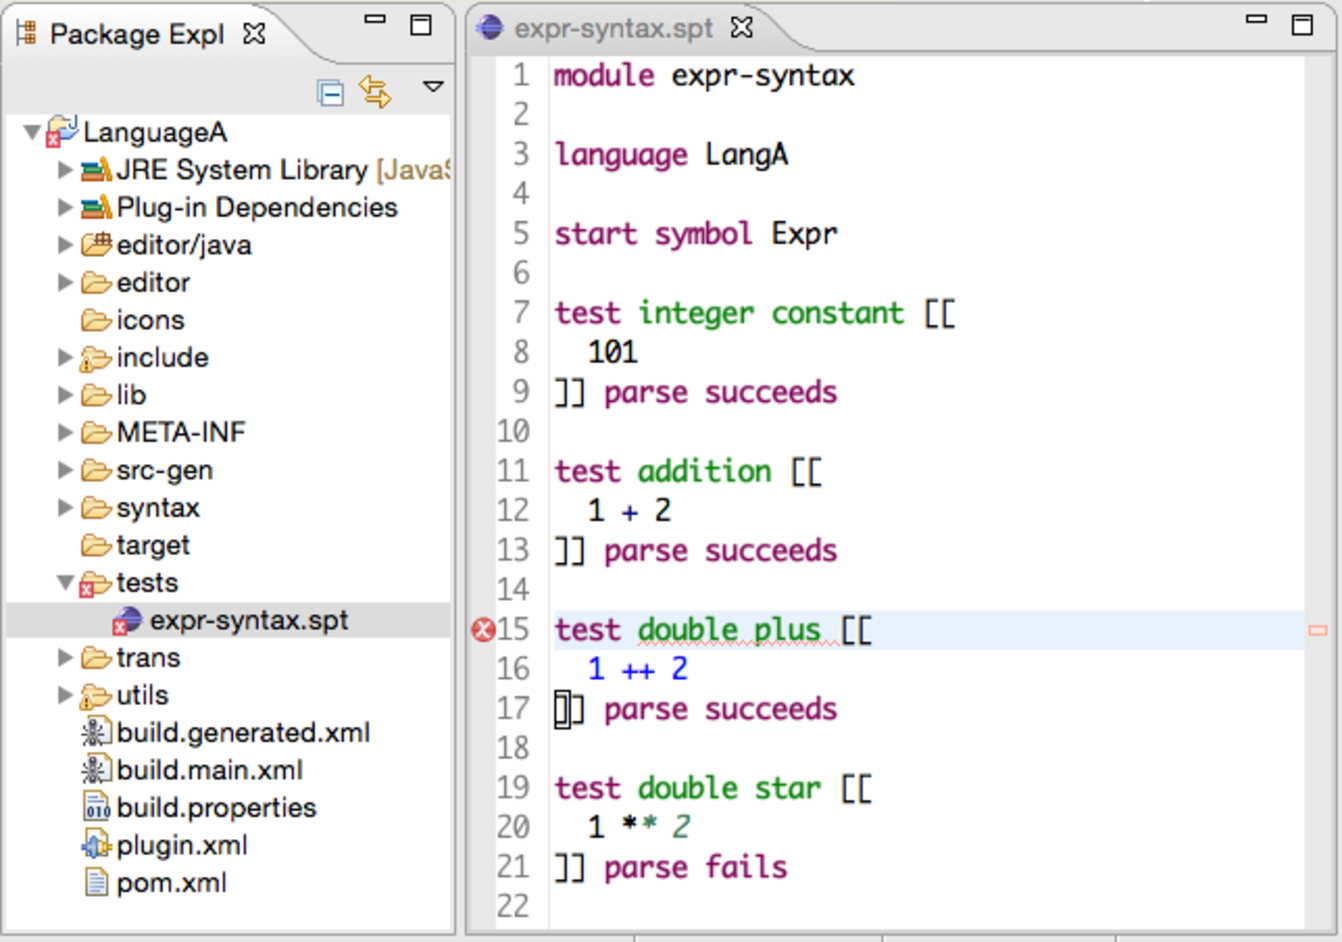
\includegraphics[width=\hsize]{tests/expr-syntax-spt.pdf}
\caption{Live evaluation of SPT test module with failing test case.}
\figurelabel{expr-syntax.spt}
\end{figure}

\Figure{class.spt} illustrates another feature of SPT. The code fragments
in a test is presented with all the features of a regular program editor.
For example, the syntax highlighting follows the syntax of the program under
test and syntax errors according to the syntax under test are hightlighted.

\begin{figure}[t]
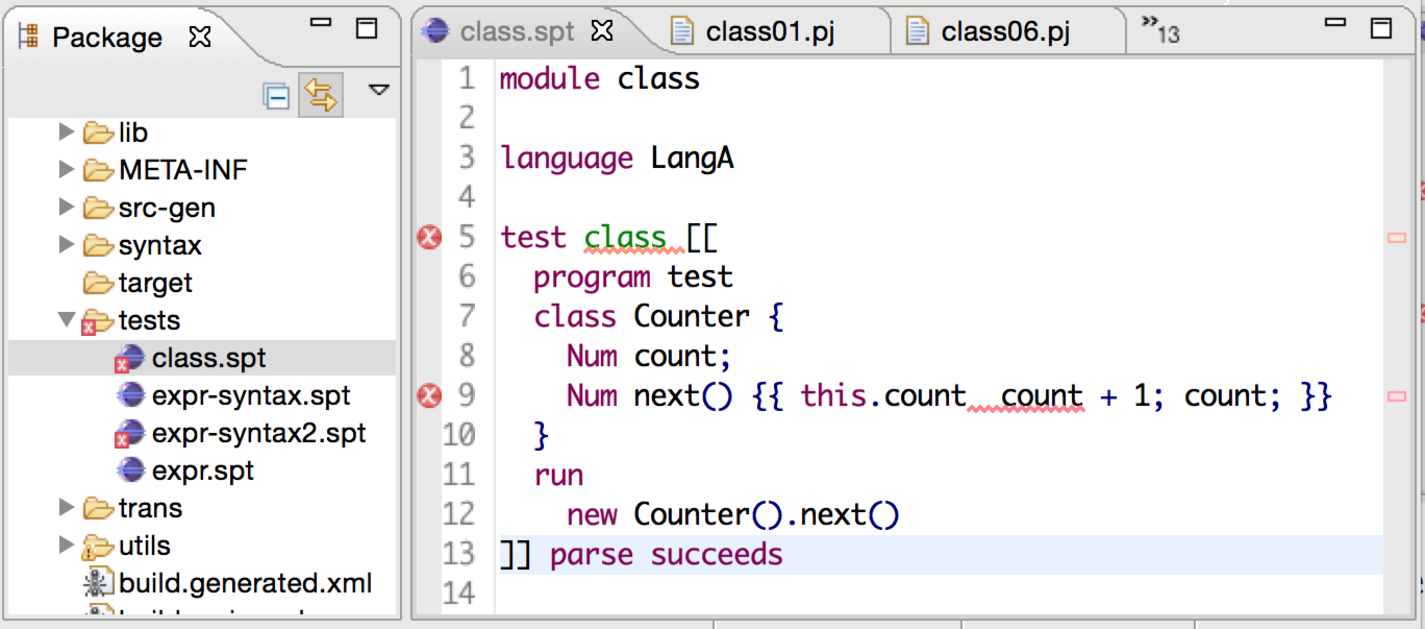
\includegraphics[width=\hsize]{tests/class-spt.pdf}
\caption{Language-specific syntax highlighting and syntax checks in test
templates.}
\figurelabel{class.spt}
\end{figure}


\section{Examples}

In addition to SPT tests, I typically maintain an \texttt{examples/} directory
with example programs in the language under development. Such examples are
useful to experience the IDE under development and exercise the various
operations being defined on programs.

\section{Further Reading}

The OOPSLA 2011 papers \cite{KatsVV11,KatsVV11a} provide a complete description
of the design and implementation of SPT.
The \href{http://metaborg.org/spt/}{SPT} page on the metaborg site provides a
complete overview of the testing features currrently supported by the
language.


